% ------------------------------------------------------------------------------
% Este fichero es parte de la plantilla LaTeX para la realización de Proyectos
% Final de Grado, protegido bajo los términos de la licencia GFDL.
% Para más información, la licencia completa viene incluida en el
% fichero fdl-1.3.tex

% Copyright (C) 2012 SPI-FM. Universidad de Cádiz
% ------------------------------------------------------------------------------

\section{Arquitectura del Sistema}
La estructura del sistema esta basada en el esquema de modelo vista controlador, introducidos en \href{http://www.codeigniter.com/}{CodeIgniter} ademas de una base de datos propia y la base de datos del media wiki, de forma que encontraremos los archivos principales en las carpetas de vista, donde se genera la interfaz para el usuario, modelo, donde se encuentran las funciones y algoritmo para el funcionamiento interno, y controladores, donde hacemos que se comuniquen las vistas con los modelos.

\subsection{Arquitectura Física}
Son necesarios para nuestro sistema un ordenador que actué de servidor (puede valer donde esté montado el Media Wiki) y el ordenador propio de los usuarios, con los cuales interactuaran con el sistema.

En principio AssessMediaWiki esta pensado para ser independiente del sistema operativo, decisión que verse afectada en un futuro dependiendo de las necesidades de escalabilidad y las funciones que se quieran implementar.

\subsection{Arquitectura Lógica}
La arquitectura del sistema se divide en las siguientes capas

\paragraph*{Modelo}
En este grupo podemos encontrar todo el software que genera las funciones para obtener, generar datos e interactuar con las bases de datos.

\paragraph*{Vista}
En este grupo podemos encontrar todo el software que genera la interfaz del usuario, siendo esta su funcionalidad exclusiva.

\paragraph*{Controlador}
Aquí encontraremos el software que completa los campos de las vistas, comunicándolas con los modelos. Los controladores se encargan de mostrar los datos del sistema en las vistas, e interaccionar con los usuarios, ya sea modificando dichos datos o navegando entre las distintas vistas.

\paragraph*{Bases de datos}
Nuestro sistema cuenta con dos bases de datos fundamentales, la base de datos del MediaWiki, donde se guarda toda la información de los alumnos y su aportación al Wiki, y la base de datos del AssessMediaWiki, donde almacenaremos la nueva información generada por la interacción de los usuarios.

\begin{figure}[h!]
	\centering
	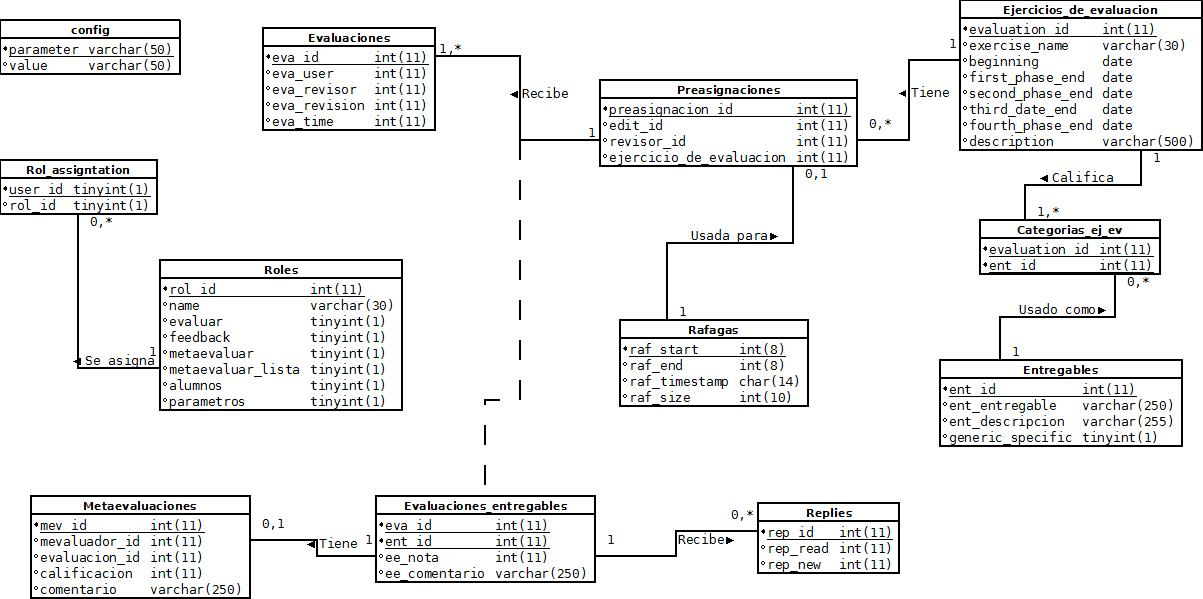
\includegraphics[width=0.9\textwidth]{db2.jpg}
	\caption{Diagrama de la base de datos de AMW 2.0.}
\end{figure}

\begin{figure}[h!]
	\centering
	\includegraphics[width=0.9\textwidth]{mediawikidb.png}
	\caption{Diagrama de la base de datos de MediaWiki (disponible en la web de MediaWiki).}
\end{figure}

\newpage

\section{Parametrización del software base}
Sera necesario editar el archivo de configuración para introducir los datos de nuestro MediaWiki, permitiendo así acceso a la base de datos y a generar las URLs para las evaluaciones (este proceso se explica detalladamente en el manual de instalación). También tenemos la opción de activar o desactivar el modo de desarrollo para hacer pruebas o cambios según se requiera.

\section{Diseño Físico de Datos}
En esta sección se define la estructura física de datos que utilizará el sistema, a partir del modelo de conceptual de clases, de manera que teniendo presente los requisitos establecidos para el sistema de información y las particularidades del entorno tecnológico, se consiga un acceso eficiente de los datos.
La estructura física se compone de tablas, índices, procedimientos almacenados, secuencias y otros elementos dependientes del SGBD a utilizar.

\begin{figure}[!h]
	\centering
	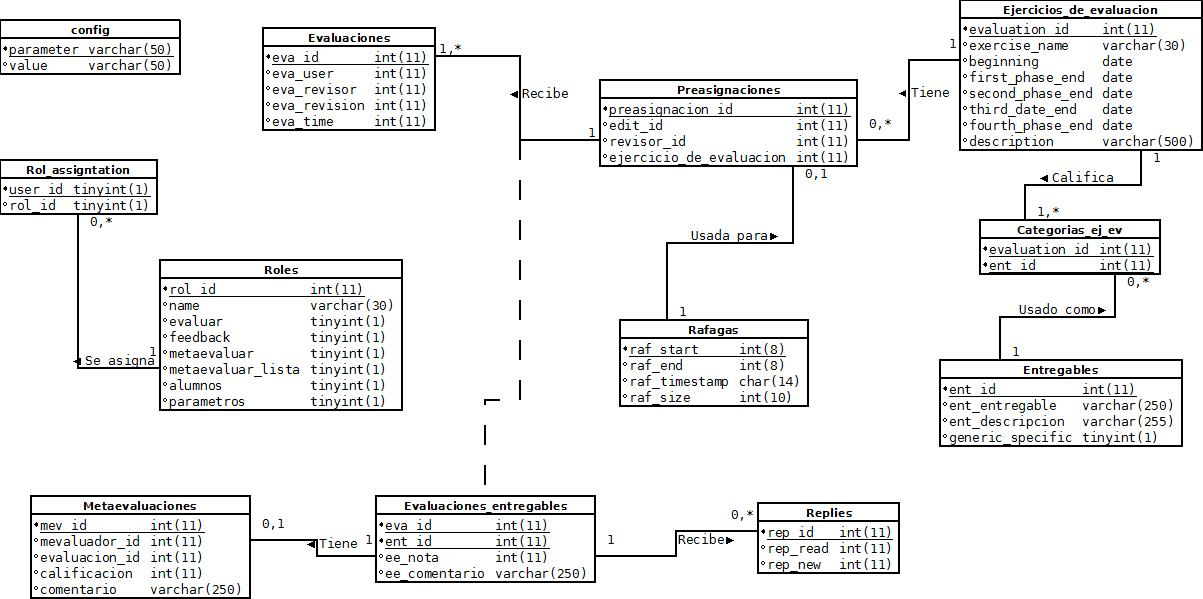
\includegraphics[width=0.9\textwidth]{db2.jpg}
	\caption{Diagrama de la base de datos de AMW 2.0.}
\end{figure}


